\documentclass[12pt]{beamer}
\usetheme{metropolis}           % Use metropolis theme
\metroset{titleformat=smallcaps}

\usepackage[utf8]{inputenc}
\usepackage[T1]{fontenc}
\usepackage{textcomp}
% \usepackage{amsmath,amsfonts,amssymb}
\usepackage{url}

% disable Navigation at the bottom
\beamertemplatenavigationsymbolsempty

% Cool font
\usepackage{FiraSans}
% \usepackage[sfdefault,light]{FiraSans}
% \usepackage{newtxsf}

% page numbers
% \setbeamertemplate{footline}[frame number]
% \setbeamertemplate{footline}
% \setbeamertemplate{headline}

% style for source code
\usepackage{listings}
\newcommand{\Hilight}{\makebox[0pt][l]{\color{light-gray}\rule[-4pt]{1.0\linewidth}{12pt}}}
\usepackage{color}
\definecolor{light-gray}{gray}{0.80}
  
% use {\mono lorem} to set something in monospace
\newcommand{\mono}[1]{\ttfamily\fontsize{14}{14}\selectfont #1}

% wanna use Metapost?
\makeatletter
\newcommand\@ptsize{12}
\makeatother

\usepackage{mflogo}
\usepackage{emp}
\DeclareGraphicsRule{*}{mps}{*}{}



\title{Disposition 1: Confidentiality}   
\author{Mathias Ravn Tversted} 
\date{\today} 


%===================================
\begin{document}

\frame{\titlepage} 

\frame{\frametitle{Table of contents}\tableofcontents} 


\frame{
    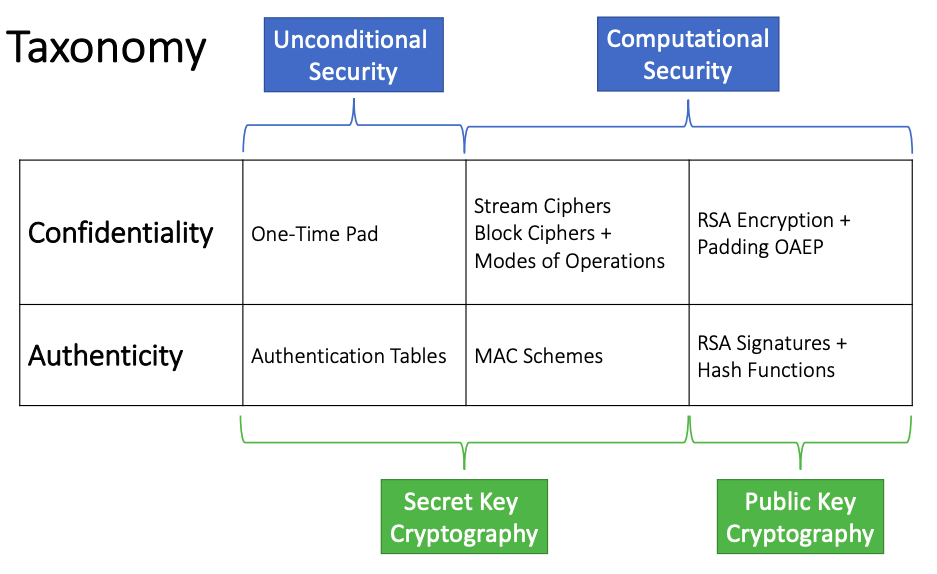
\includegraphics[width=\linewidth]{content/taxanomy.png}
}


%===================================
\section{Unconditional security} 

\frame{\frametitle{Perfect Secrecy: One-time Pad}
    One-time pad relies on the following identity
    \begin{align*}
        c_i \bigoplus k_i = (m_i \bigoplus k_i) \bigoplus k_i = m_i \bigoplus (k_i \bigoplus k_i) = m_i
    \end{align*}
    And has perfect secrecy\footnote{Theorem 5.1}.
    The cipher text does not rely on the distribution of the message, but you need a key size that is at least as long as the cipher text, and is therefore not really useful in practice.
}


\section{Computational security, Secret-key systems}
\subsection{Definition of security}
\frame{\frametitle{Definition of security}
    We consider a case of an oracle with the secret-key, which either spits out $c = E_k(m, n)$ or $E_k(r, n)$. So either a random message or the message encrypted with a nonce.

    Downside is that all parties must have the secret key. 

    \textbf{Definition 5.3:} Consider any adversary who plays the above game, and whose computing power is limited in the sense that whatever algorithm he runs terminates in time much less than the time it takes to try all possible keys the cryptosystem. No such adversary can guess whether he is in case 1 or 2 with probability better than a random guess.
}    

\subsection{Stream ciphers/Block ciphers}
\frame{\frametitle{Stream Ciphers}
    An algorithm $X$, which expends a short key $k$, and a nonce $n$ to a longer \textit{looking} string $X(k, n)$. Which is then used to encrypt a message \textit{as if} it was a one-time pad. That is, $c = m \bigoplus X(k, n)$. Decryption happens with $c = \bigoplus X(k, n) = m \bigoplus X(k, n) \bigoplus X(k, n) = m$.   

    Stream algorithms do not produce truly random outcomes. We cannot output more than $2^{length}$ different strings. (TJEK DET HER FARMAND SIDE 130) 
}

\frame{\frametitle{Stream Ciphers}
    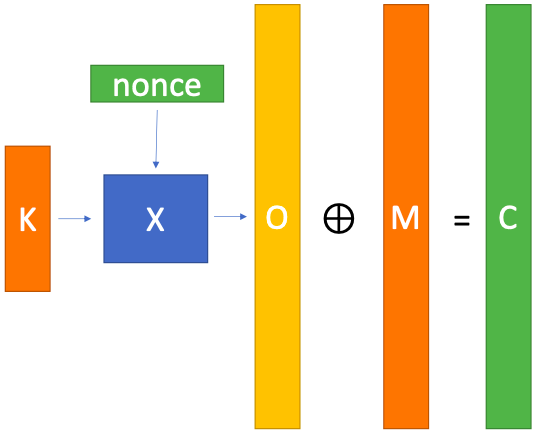
\includegraphics[width=\linewidth]{content/stream-cipher-enc.png}
}

\frame{\frametitle{Block ciphers}
    Block ciphers encrypt a fixed size block of data, and outputs a block of the same size. Block ciphers have \textit{modes of operation} (such as Cipher Block Chaining, Counter \& Output feedback). 

    They have a \textit{nonce}, which is called an \textit{Initialisation Vector}. This must be chosen carefully and not be the same all the time. 

    \textbf{Examples:} 1. DES (56 bit keys, 64-bit blocks) 2. Triple-DES (112 or 168-bit keys, 64-bit blocks). 3. AES (HVAD ER SPECI?)
}
\subsection{CBC/CTR/OFB modes}
\frame{\frametitle{OFB: Output Feedback}
    Generate a keystream. Take a nonce $IV$, then apply AES to it repeatedly. 
    \begin{align*}
        AES_K(IV), AES_K(AES_K(IV)), ...,
    \end{align*}
    Then we can XOR that with the message. 
}
\frame{
    \frametitle{CBC: Cipher Block Chaining}
        CBC is more common. Let the message consist of 128-bit blocks $M_1, ..., M_t$, we pad the last block. The cipher text will be $t + 1$ blocks $C_0, ..., C_t$ where $C_0 = IV$ and for $i = 1, ..., t$
        \begin{align*}
            C_i = AES_k(M_i \bigoplus C_{i - 1})
        \end{align*}
        The $IV$ must be random to satisfy \textit{indistinguishability under chosen-plaintext}. $IV$ cannnot be implemented as a counter in CBC mode. (EXPLAIN!!!)
}

\frame{
    \frametitle{CBC: Cipher Block Chaining}
    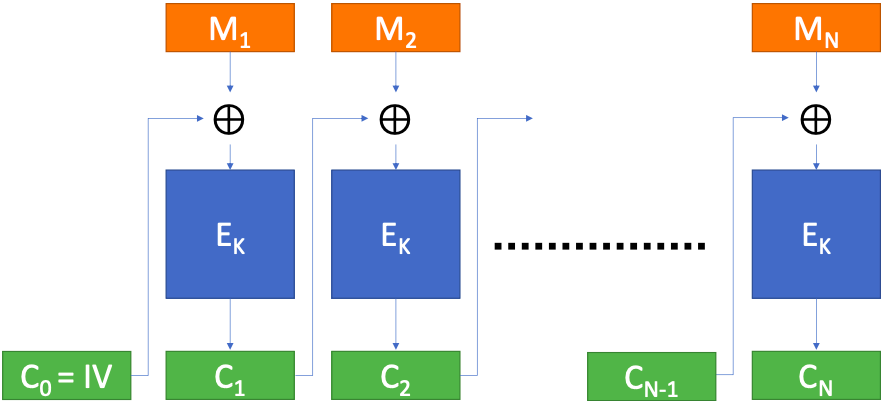
\includegraphics[width=\linewidth]{content/cbc-enc.png}
}

\frame{
    \frametitle{CTR: Counter Mode}
        Let the message be $M_1, ..., M_t$ and the ciphertext depending on $IV$. The cipher text will be $t + 1$ blocks $C_0, ..., C_t$ where $C_0 = IV$ and for $i = 1, ..., t$
        \begin{align*}
            C_i = AES_K(IV + i) \bigoplus M_i
        \end{align*}
        $IV + 1$ means that $IV$ is a 128-bit number. Add $i \text{ mod }2^{128}$. CTR makes it easier to decrypt several blocks than CBC in parallel. 
}

\frame {
    \frametitle{CTR: Counter Mode}
    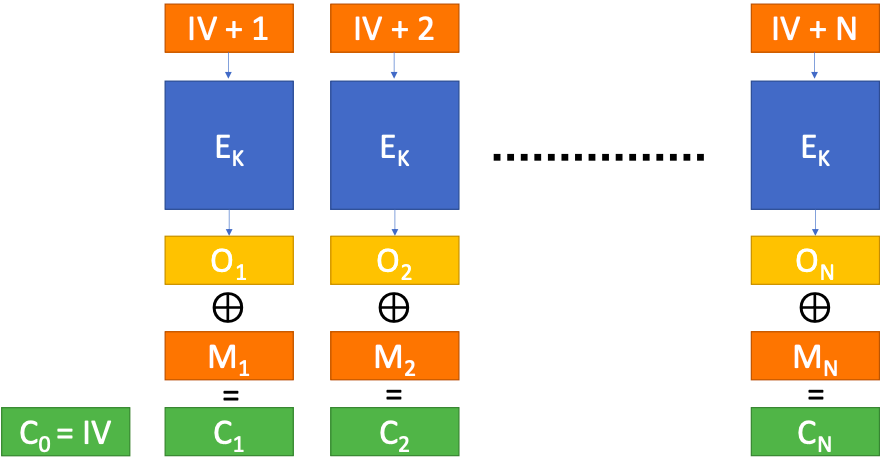
\includegraphics[width=\linewidth]{content/ctr-enc.png}
}

\section{Computational Security, public-key systems}
\frame{\frametitle{Public-key Systems}
    Public-key systems also have three algorithms. $G, E, D$. Algorithm $G$ has input key of length $\kappa$ and outputs a pair of keys of length $\kappa$. Public key makes use of two matching keys, instead of one. It uses the following identity
    \begin{align*}
        m = D_{sk}(E_{pk}(m))
    \end{align*}
    Secret-key systems also require the use of randomness. Otherwise they could win the oracle game. 
}
\subsection{RSA, AES, OAEP}
\frame{\frametitle{AES}
    MISSING????
}

\frame{\frametitle{RSA}
    Relies on difficulty of prime factorisation.  
    Let $N, e$ be the public key. Let $n, d$ be the private key. $N = p \cdot q$. Let $d = f(e, p, q)$.  Below is the deterministic and thus insecure vanilla RSA. It relies on the following identity. Here $c = m^e \text{ mod } n$. 
    \begin{align*}
        c^d \text{ mod } n = (m^e \text{ mod } n)^d \text{ mod } n = m
    \end{align*}
    Size of keys must be big (2-3k bits), and can just grow. 
    Let $d = e^{-1} \text{ mod } (p - 1)(q-1)$. RSA is commonly used.
}
\frame{\frametitle{OAEP}
    1. Compute a padded version $OAEP(K, R)$. $R$ is a random string of bits. $|R|$ is chosen as a function of $N$. 
    2. Ciphertext is $c = OAEP(K, R)^e \text{ mod } n$. 
    3. Receiver computes $(OAEP(K, R)^e \text{ mod } n)^d = OAEP(K, R)$ Check that the format of the result is correct, and if so, receiver recovers $K$ from $OAE(K, R)$. Chose $OAEP$ such that this is possible. 
}


\end{document}

